\section{Kiến trúc Hệ thống Tổng thể}
\label{sec:kientruc_tongthe}

\subsection{Cấu trúc Phân tầng Clean Architecture Phía Client}
Ứng dụng di động MyHCMUT được thiết kế theo mô hình Clean Architecture phân tách rõ rệt 3 tầng:

\begin{figure}[H]
    \centering
    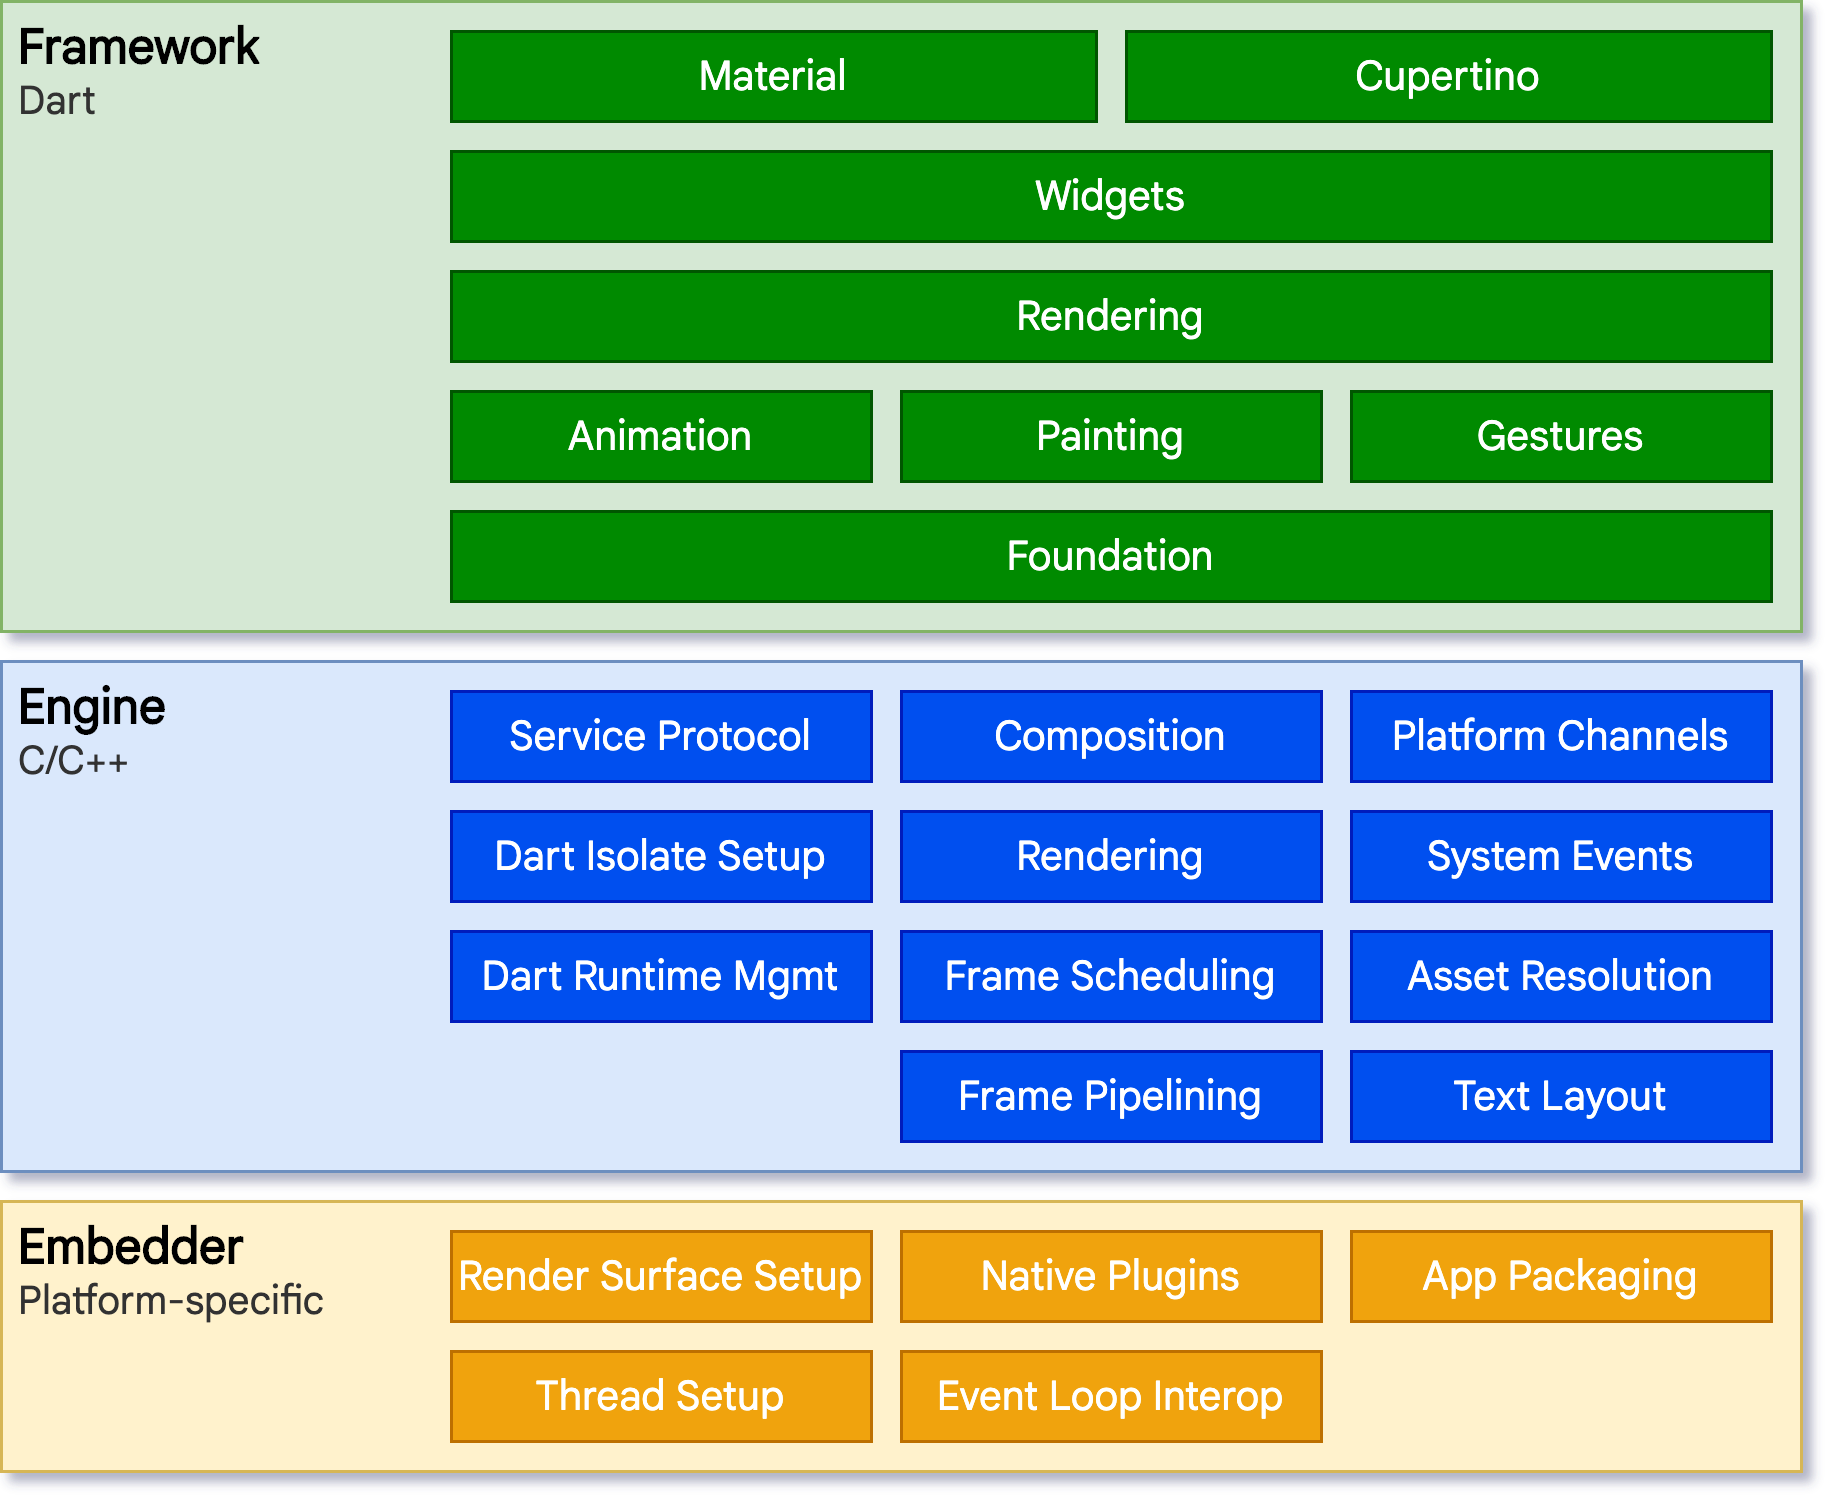
\includegraphics[width=0.9\linewidth]{img/architecture/mobile_clean_architecture.png}
    \caption{\textit{Kiến trúc Phân tầng Clean Architecture của Ứng dụng MyHCMUT}}
    \label{fig:mobile_clean}
\end{figure}

\begin{itemize}
    \item \textbf{Tầng Trình diễn (Presentation Layer):} Pages, Widgets và Riverpod Notifiers quản lý trạng thái phản ứng giao diện (\texttt{AsyncValue}).
    \item \textbf{Tầng Nghiệp vụ (Domain Layer):} Entities, Freezed DTOs và quy tắc nghiệp vụ client (Form Wizard State, Validation).
    \item \textbf{Tầng Dữ liệu (Data Layer):} Repositories, Dio Data Sources, SQLite Local Cache và Secure Storage.
\end{itemize}

\subsection{Hệ thống Giao diện Material 3 Semantic Tokens (\texttt{global\_system})}
Chuẩn hóa bảng màu, kiểu chữ, khoảng cách và các widget tái sử dụng (\texttt{AppBatchActionBar}, thẻ Card, Badges trạng thái) theo Semantic Tokens, đảm bảo tương thích 100\% giữa Light Mode và Dark Mode.

\subsection{Thiết kế Bộ điều phối Token Đa miền (\texttt{MultiDomainAuthInterceptor})}
\begin{itemize}
    \item Tự động trích xuất chuỗi JWT \texttt{token\_auth} từ \texttt{flutter\_secure\_storage}.
    \item Tự động gắn tiêu đề \texttt{Authorization: Bearer <token>} vào mọi request gửi tới các Backend (\texttt{myhcmut-be}, \texttt{hrm-be}, \texttt{ioffice-be}).
    \item Lắng nghe phản hồi HTTP 401: Tự động kích hoạt luồng Silent Refresh Token ở tầng nền và phát lại request gốc mà không làm gián đoạn trải nghiệm người dùng.
\end{itemize}

\subsection{Thiết kế Dữ liệu Thông báo Đẩy có Cấu trúc (Structured Metadata Routing)}
Loại bỏ việc bóc tách chuỗi URL không ổn định, thiết kế cấu trúc payload gồm 4 trường Metadata có cấu trúc:
\begin{itemize}
    \item \texttt{source}: Phân hệ phát sinh thông báo (\texttt{'hrm'} / \texttt{'ioffice'}).
    \item \texttt{entityType}: Loại đối tượng (\texttt{'leave'}, \texttt{'business-trip'}, \texttt{'incoming-doc'}, \texttt{'outgoing-doc'}, \texttt{'task'}).
    \item \texttt{entityId}: ID bản ghi nghiệp vụ cụ thể.
    \item \texttt{isApproval}: Cờ đánh dấu màn hình duyệt dành cho cấp quản lý (\texttt{'true'} / \texttt{'false'}).
\end{itemize}
Lớp \texttt{NotificationRouteParser} phân tích trực tiếp 4 trường này để kích hoạt \texttt{GoRouter} điều hướng sâu (Deep Linking) chính xác vào màn hình chi tiết.
